\documentclass[english]{article}

%% Packages pull in extra commands:
%% http://en.wikibooks.org/wiki/LaTeX/Packages

\usepackage{hyperref}
\usepackage[letterpaper]{geometry}
\geometry{verbose,tmargin=1in,bmargin=1in,lmargin=1in,rmargin=1in}
\usepackage{amsmath}
\usepackage{amssymb}
\usepackage{graphicx}
\usepackage{float}
\usepackage{array}
\usepackage{tikz}
\usepackage{enumitem}
\usepackage{bbm}
\usepackage{xspace}
\DeclareMathOperator*{\argmax}{argmax}
\usepackage{spverbatim}

% New commands serve as shorthand for frequently used command combinations.
\newcommand{\ind}[1]{\mathbf{1}\left(#1\right)}
\newcommand{\bx}{\mathbf{x}}
\newcommand{\E}{\mathbf{E}}
\newcommand{\MATLAB}{\textsc{Matlab}\xspace}
\newcommand\scalemath[2]{\scalebox{#1}{\mbox{\ensuremath{\displaystyle #2}}}}

\title{CIS581: Computer Vision and Computational Photography\\Final Project\\Final Project Proposal}
\author{%
 \begin{tabular}{rl}
 Tianlin Du&(dtl1995) \tabularnewline
  Wentao He&(wentaoh) \tabularnewline
  Yezheng Li&(yezheng)
\end{tabular}
}

\begin{document}
\maketitle

\section{Overview}
In this (short) project, we will implement vanilla recurrent neural networks (RNNs) and Long-Short Term Memory (LSTM) RNNs and apply them to image captioning on COCO.\\\\
Note: this project is adapted from the Standford CS231n course.

\section{Goal}
We will take a look at an interesting multi-modal topic where we will combine both image and text processing to build a useful Deep Learning application, aka Image Captioning. Image Captioning refers to the process of generating textual description from an image based on the objects and actions in the image.\\\\
Here are some examples of image captioning:\\\\
        \begin{figure}[H]
          \centering
          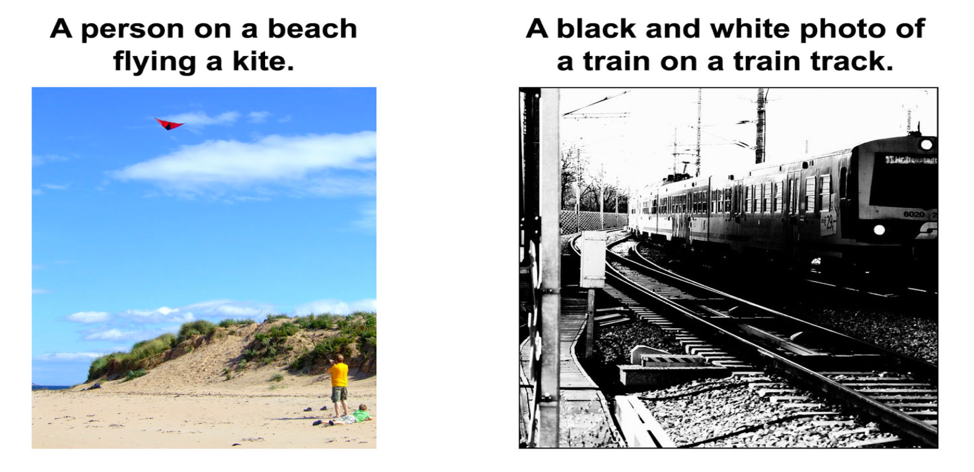
\includegraphics[width=0.8\textwidth]{Picture1.png}
          \caption{}
        \end{figure}
        \begin{figure}[H]
          \centering
          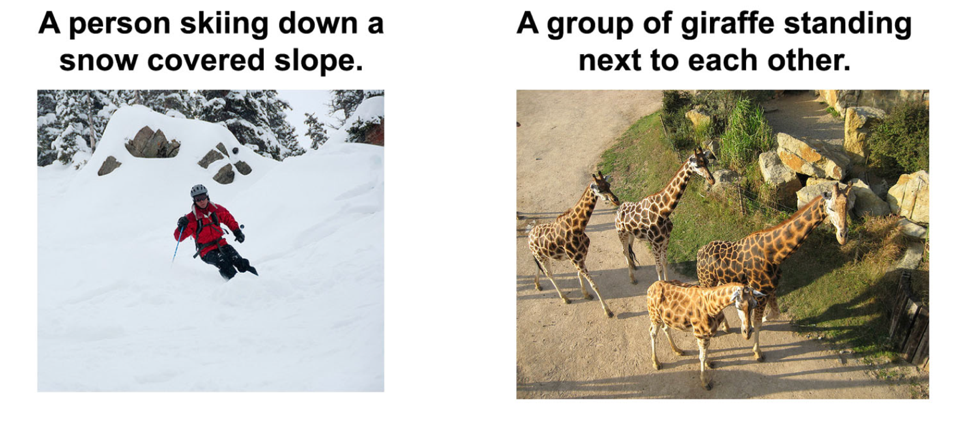
\includegraphics[width=0.8\textwidth]{Picture2.png}
          \caption{}
        \end{figure}
A TensorFlow implementation of the image-to-text model described in the paper: "\textit{Show and Tell: Lessons learned from the 2015 MSCOCO Image Captioning Challenge.}" Full text is available at: \url{http://arxiv.org/abs/1609.06647}.

\section{Architecture}
The Show and Tell model is an example of an encoder-decoder neural network. It works by first "encoding" an image into a fixed-length vector representation, and then "decoding" the representation into a natural language description.\\\\
The image encoder is a deep convolutional neural network. This type of network is widely used for image tasks and is currently
state-of-the-art for object recognition and detection. Our particular choice of network is the Inception v3 image recognition model
pretrained on the ILSVRC-2012-CLS image classification dataset.\\\\
The decoder is a long short-term memory (LSTM) network. This type of network is commonly used for sequence modeling tasks such as
language modeling and machine translation. In the Show and Tell model, the LSTM network is trained as a language model conditioned on
the image encoding. Words in the captions are represented with an embedding model. Each word in the vocabulary is associated with a fixed-length vector representation that is learned during training.\\\\
The following diagram illustrates the model architecture. In this diagram, $S_0, S_1, \cdots, S_{N-1}$ are the words of the caption and $W_eS_0, W_eS_1, \cdots, W_eS_{N-1}$ are their corresponding word embedding vectors. The outputs $p_1, p_2, \cdots, pN$ of the LSTM are probability distributions generated by the model for the next word in the sentence. The terms $\log p_1(S1), \log p_2(S_2), \cdots, \log p_N(S_N)$ are the log-likelihoods of the correct word at each step; the negated sum of these terms is the minimization objective of the model.\\\\
During the first phase of training the parameters of the Inception v3 model are kept fixed: it is simply a static image encoder function. A single trainable layer is added on top of the Inception v3 model to transform the image embedding into the word embedding vector space. The model is trained with respect to the parameters of the word embeddings, the parameters of the layer on top of Inception v3 and the parameters of the LSTM. In the second phase of training, all parameters - including the parameters of Inception v3 - are trained to jointly fine-tune the image encoder and the LSTM.\\\\
\begin{figure}[H]
          \centering
          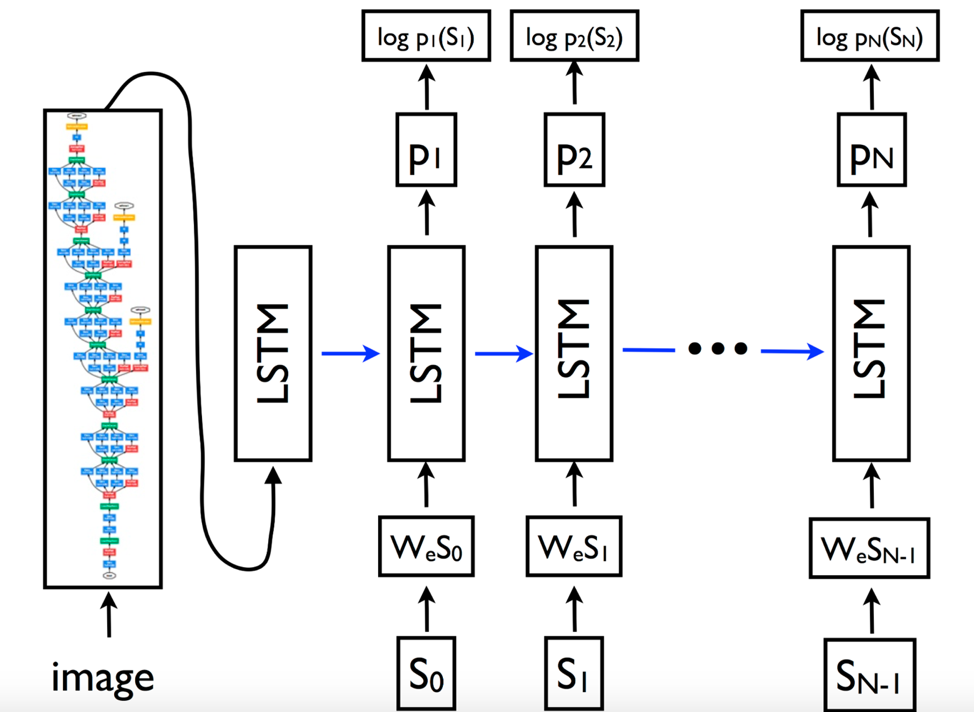
\includegraphics[width=0.8\textwidth]{Picture3.png}
          \caption{Picture1}
\end{figure}

Given a trained model and an image we use beam search to generate captions for that image. Captions are generated word-by-word, where at each step $t$ we use the set of sentences already generated with length $t - 1$ to generate a new set of sentences with length $t$. We keep only the top k candidates at each step, where the hyperparameter $k$ is called the beam size. We have found the best performance with k = 3.

\section{Part 1}
Open the \texttt{RNN\_Captioning.ipynb} in Jupyter notebook, which will walk you through implementing the forward and backward pass for a vanilla RNN, first, 1) for a single timestep and then, 2) for entire sequences of data. Code to check gradients has already been provided. \\\\You will overfit a captioning model on a tiny dataset and implement sampling from the softmax distribution and visualize predictions on the training and validation sets.

\section{Part 2}
Open the \texttt{LSTM\_Captioning.ipynb} Jupyter notebook, which will walk you through the implementation of Long-Short Term Memory (LSTM) RNNs, and apply them to image captioning on MS-COCO.

\section{Part 3}
Using the pieces you implement in parts 1 and 2, train a captioning model that gives decent qualitative results (better than the random garbage you saw with the overfit models) when sampling on the validation set.\\\\
Code for evaluating models using the BLEU unigram precision metric has already been provided. Feel free to use PyTorch for this section if you’d like to train faster on a GPU.\\\\
Here are a few pointers:\\
\begin{enumerate}
\item Attention-based captioning models. \textit{[1, 7] Show, Attend and Tell: Neural Image Caption Generation with Visual Attention. Xu et al., 2015}. \url{https://arxiv.org/abs/1502.03044}.
\item \textit{Knowing When to Look: Adaptive Attention via A Visual Sentinel for Image Captioning. Lu et al., CVPR 2017}. \url{https://arxiv.org/abs/1612.01887}.
\item Discriminative captioning. \textit{Context-aware Captions from Context-agnostic Supervision. Vedantam et al., CVPR 2017}. \url{https://arxiv.org/abs/1701.02870}.
\item Novel object captioning. \textit{Deep Compositional Captioning: Describing Novel Object Categories without Paired Training Data. Hendricks et al., CVPR 2016}. \url{https://arxiv.org/abs/1701.02870}.
\item \textit{Captioning Images with Diverse Objects. Venugopalan et al., CVPR 2017}. \url{https://arxiv.org/abs/1701.02870}.
\end{enumerate}
\section{Deliverables}
Submit the notebooks and code you wrote with all the generated outputs. Run \texttt{collect\_submission.sh} to generate the zip file for submission.

\section{References}
\begin{enumerate}
    \item Automatic Image Captioning using Deep Learning (CNN and LSTM) in PyTorch. \url{https://www.analyticsvidhya.com/blog/2018/04/solving-an-image-captioning-task-using-deep-learning/}.
    \item \url{https://github.com/tensorflow/models/tree/master/research/im2txt}.
    \item CS231n Convolutional Neural Networks for Visual Recognition. \url{http://cs231n.github.io/assignments2017/assignment3/}.
    \end{enumerate}

\end{document}
